\documentclass[conference]{IEEEtran}
\IEEEoverridecommandlockouts
% The preceding line is only needed to identify funding in the first footnote. If that is unneeded, please comment it out.
\usepackage{cite}
\usepackage[ngerman]{babel}
\usepackage[utf8]{inputenc}
\usepackage{amsmath,amssymb,amsfonts}
\usepackage{algorithmic}
\usepackage{graphicx}
\usepackage{textcomp}
\usepackage{xcolor}
\usepackage{listings}


\definecolor{pblue}{rgb}{0.13,0.13,1}
\definecolor{pgreen}{rgb}{0,0.5,0}
\definecolor{pred}{rgb}{0.9,0,0}
\definecolor{pgrey}{rgb}{0.46,0.45,0.48}
\lstset{language=Python,
	showspaces=false,
	showtabs=false,
	breaklines=true,
	tabsize=2,
	showstringspaces=false,
	breakatwhitespace=true,
	commentstyle=\color{pgreen},
	keywordstyle=\color{pblue},
	stringstyle=\color{pred},
	basicstyle=\ttfamily
}


\usepackage{url}
\def\BibTeX{{\rm B\kern-.05em{\sc i\kern-.025em b}\kern-.08em
		T\kern-.1667em\lower.7ex\hbox{E}\kern-.125emX}}
\begin{document}
	
	\title{Videoanalyse und Objekttracking}
	
	\author{\IEEEauthorblockN{1\textsuperscript{st} Bartolovic Eduard}
	\IEEEauthorblockA{\textit{Hochschule München} \\
		München, Deutschland \\
		eduard.bartolovic0@hm.edu}
	\and
	\IEEEauthorblockN{2\textsuperscript{nd} Thomas Willeit}
	\IEEEauthorblockA{\textit{Hochschule München} \\
		München, Deutschland \\
		XXXXX@hm.edu}
	\and
	\IEEEauthorblockN{3\textsuperscript{rd} Schäfer Julia}
	\IEEEauthorblockA{\textit{Hochschule München} \\
		München, Deutschland \\
		j.schaefer0@hm.edu}
	}

	
	\maketitle
	
	\begin{abstract}
		
	\end{abstract}
	
	
	\section{Videomaterial}
	Für dieses Projekt wurden mehrere Aufnahmen aufgenommen.\\ Ziel war es keine zu chaotischen aber auch nicht zu einfache Aufnahmen zu erstellen. Auch sollten verschiedene Szenarien abgebildet werden.\\
	\textbf{Verkehrsaufnahmen am Brudermühltunnel am Mittleren Ring.} Dieser Teil ist sehr verkehrsreich und Autobahnähnlich ausgebaut. Es gibt mehrere Fahrspuren. Alle Fahrzeuge fahren in eine Richtung. Es sind ein paar Laternen und Bäume in der Aufnahme. Es sind nur Pkw und kleine Transporter welche trotzdem als Pkw klassifiziert werden enthalten.
	\begin{figure}[!h]
		\begin{center}
			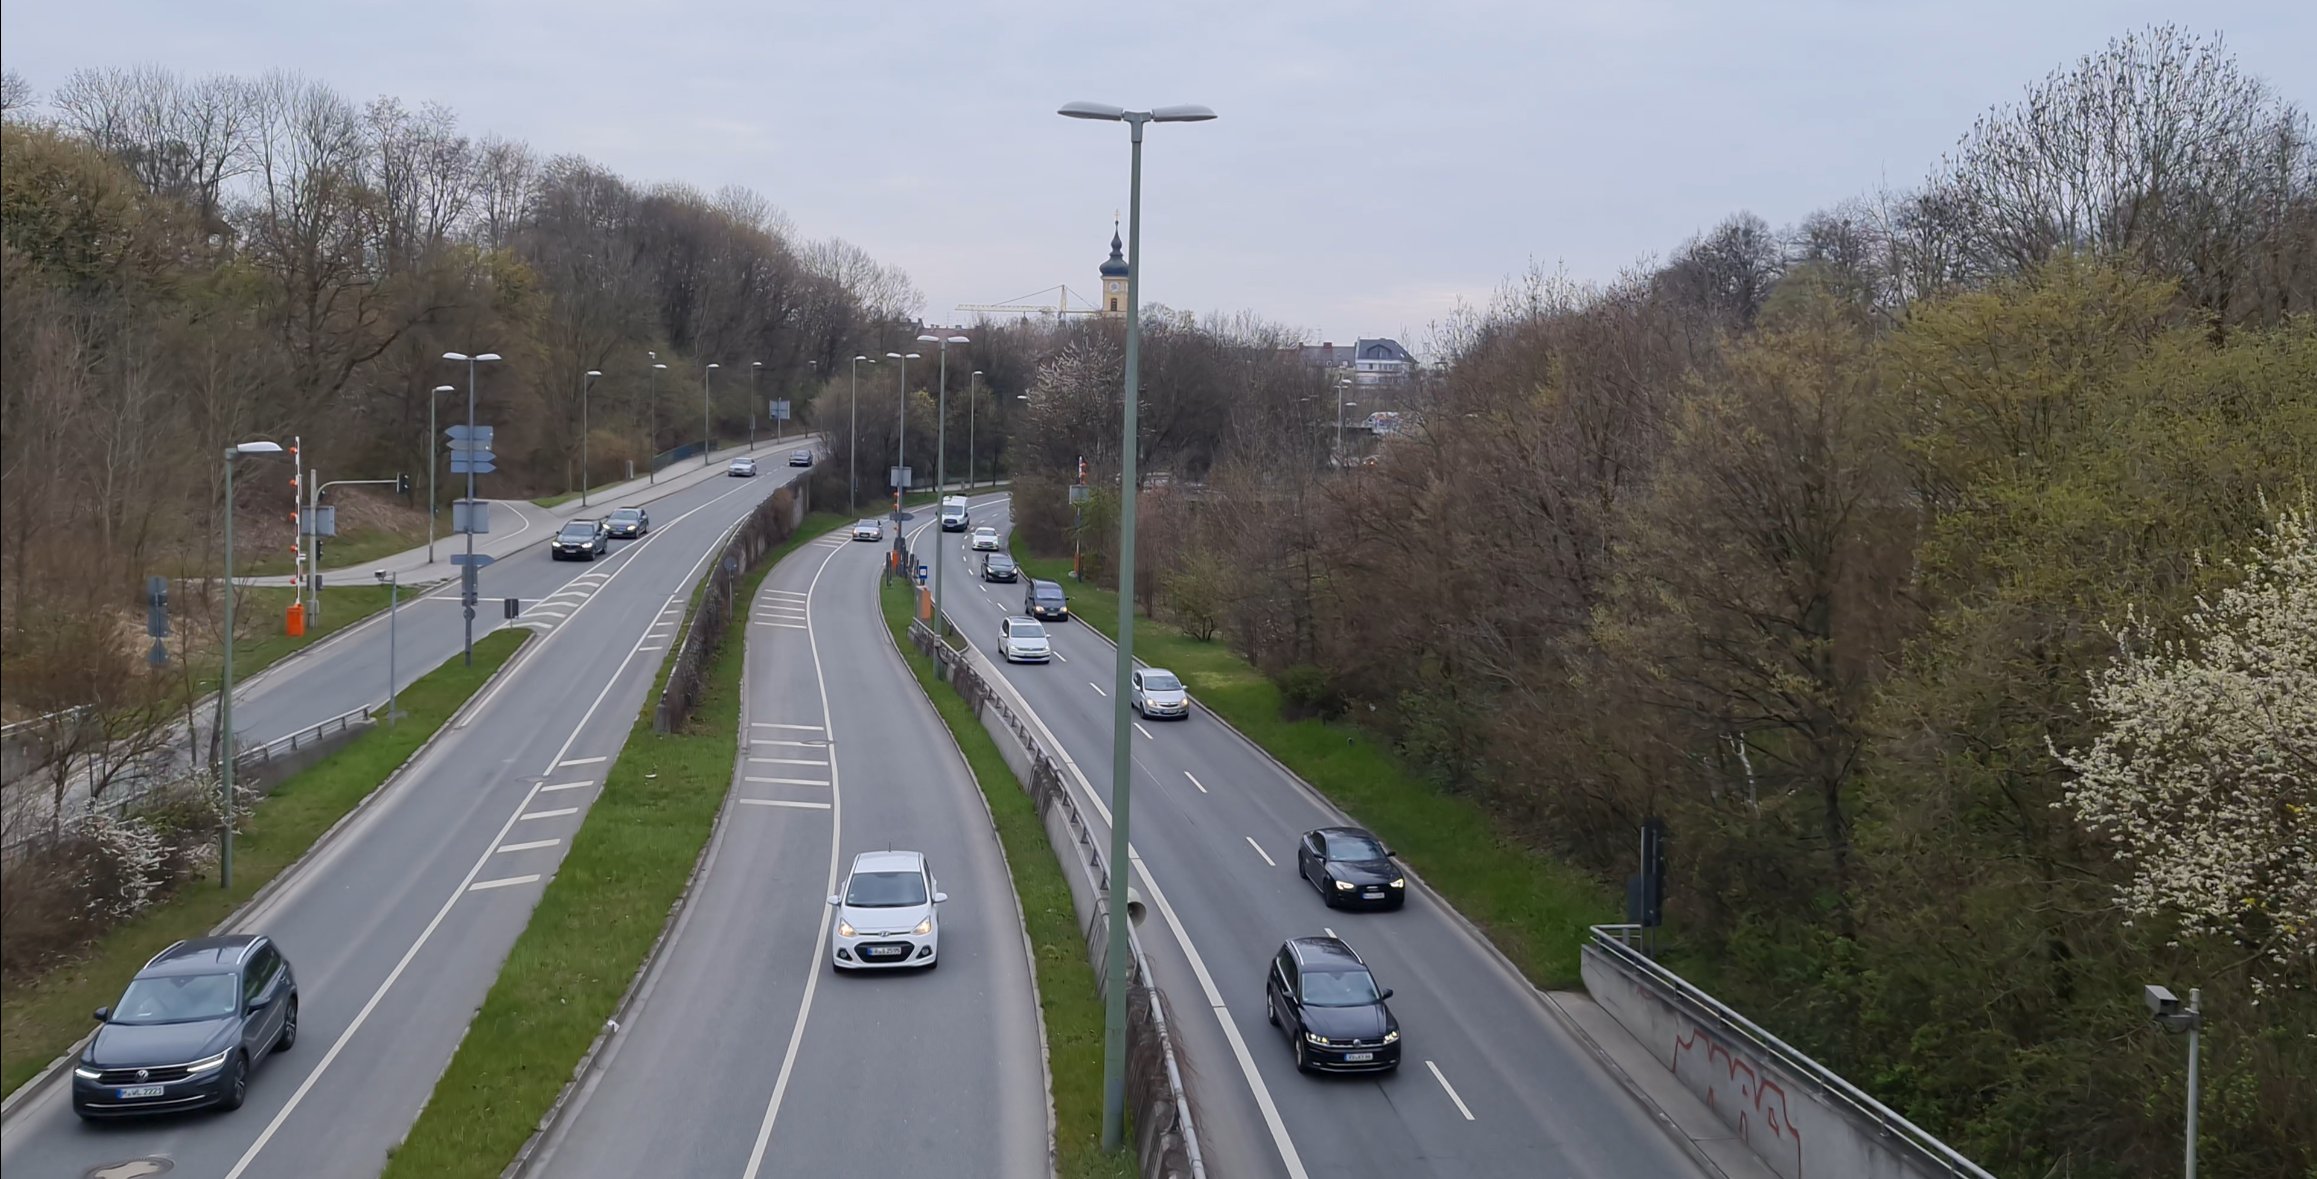
\includegraphics[width=7cm]{Media/BrudermuhlRaw.png}
			\caption{Verkehrsaufnahmen am Brudermühltunnel}
			\label{BrudermuhlRaw}
		\end{center}
	\end{figure}\\
	\textbf{Verkehrsaufnahmen am Candidtunnel.} Eine stark befahrene Straße mit einer viel zahl von Verkehrsteilnehmern. Es herrscht zwei Richtungsverkehr mit insgesamt 4 Fahrspuren. In eine Richtung stehen die Fahrzeuge in einem Stau. Durch Regen spiegeln viele Oberflächen. Die Bäume bewegen sich aufgrund von stärkeren Wind. Diese Aufnahme ist die anspruchsvollste. In diesem Video sind neben Pkw auch Busse enthalten.
	\begin{figure}[!h]
		\begin{center}
			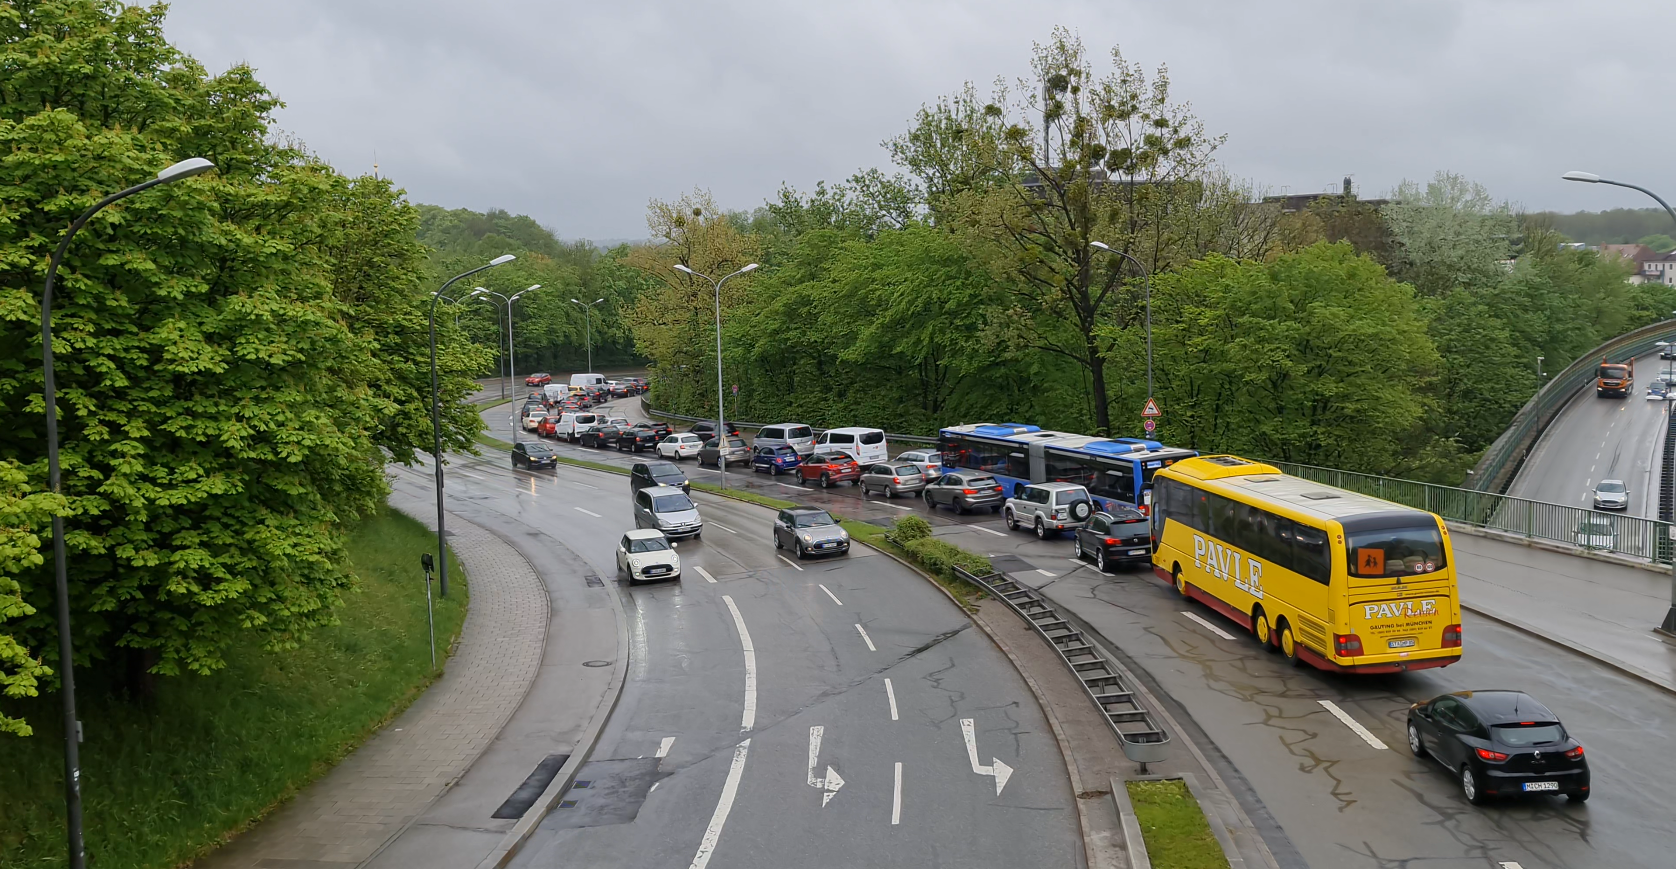
\includegraphics[width=7cm]{Media/CandidRaw.png}
			\caption{Verkehrsaufnahmen am Candidtunnel.}
			\label{BrudermuhlRaw}
		\end{center}
	\end{figure}\\
	\textbf{Zugaufnahmen an der Donnersbergerbrücke.} Eine Aufnahme der am stärksten befahren Bahnstrecken Europas \cite{z1}. Hier existiert viel Zugverkehr auf mehreren Gleisen mit unterschiedlichen Zugtypen. Beobachtet werden die vier Gleise der zwei Bahnsteige der S-Bahnhalt \textit{Donnersbergerbrücke}. Ein Hindernis sind die Masten, Signale und das Bahnsteigdach welche einen einen guten Blick auf die Züge erschweren. In dieser Aufnahme sind Züge und Fußgänger enthalten.
	\begin{figure}[!h]
		\begin{center}
			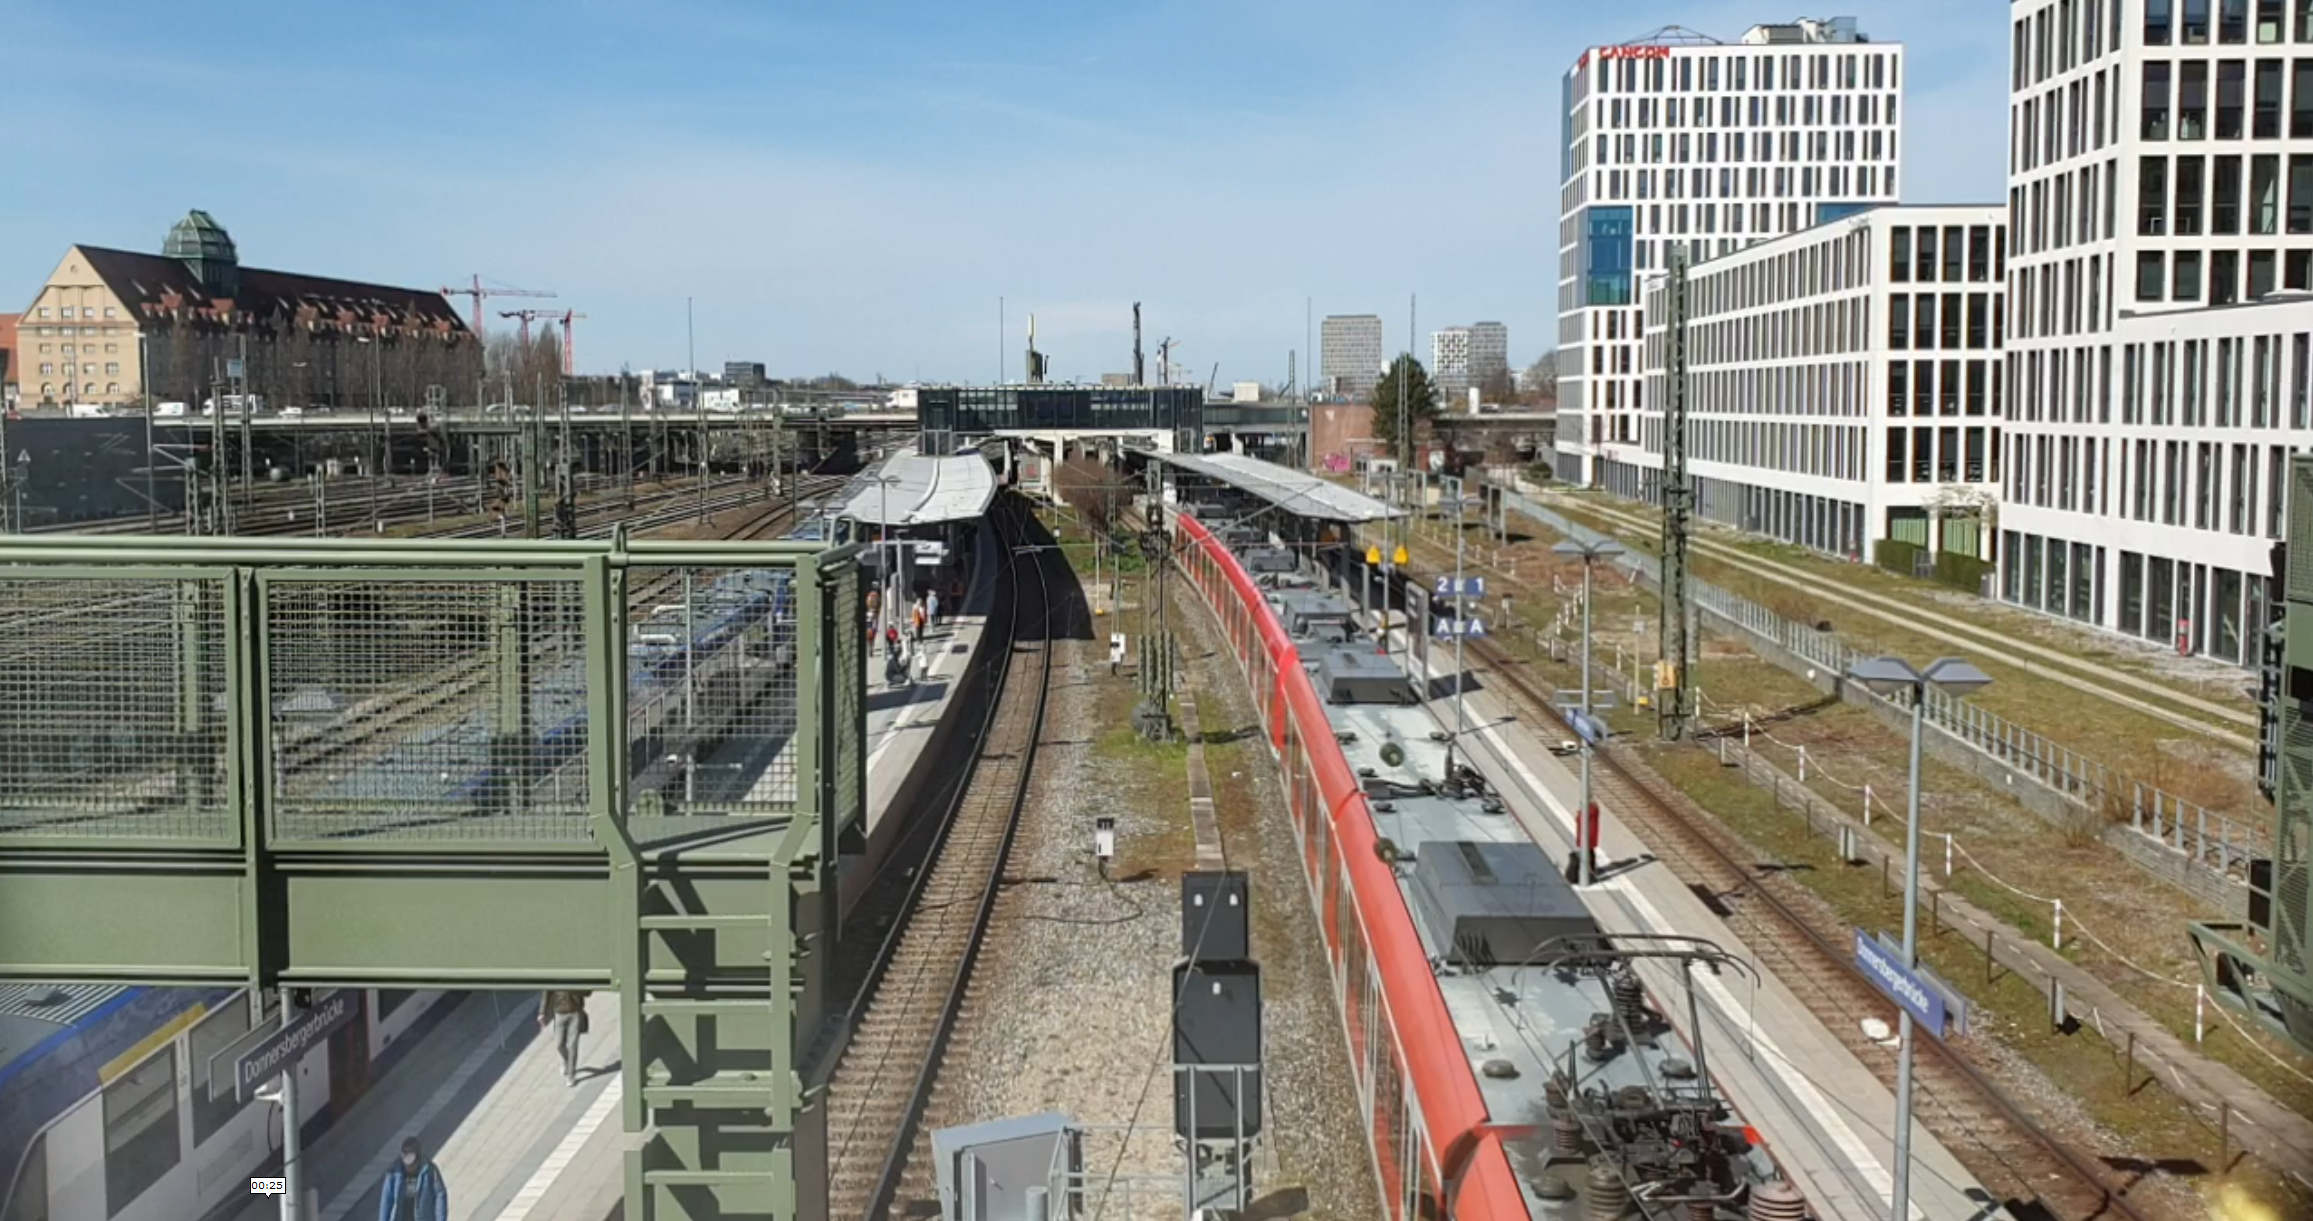
\includegraphics[width=7cm]{Media/DonnersbergerRaw.png}
			\caption{Zugaufnahmen an der Donnersbergerbrücke}
			\label{BrudermuhlRaw}
		\end{center}
	\end{figure}


	\section{Konzept}
	
	\begin{figure*}[!h]
		\begin{center}
			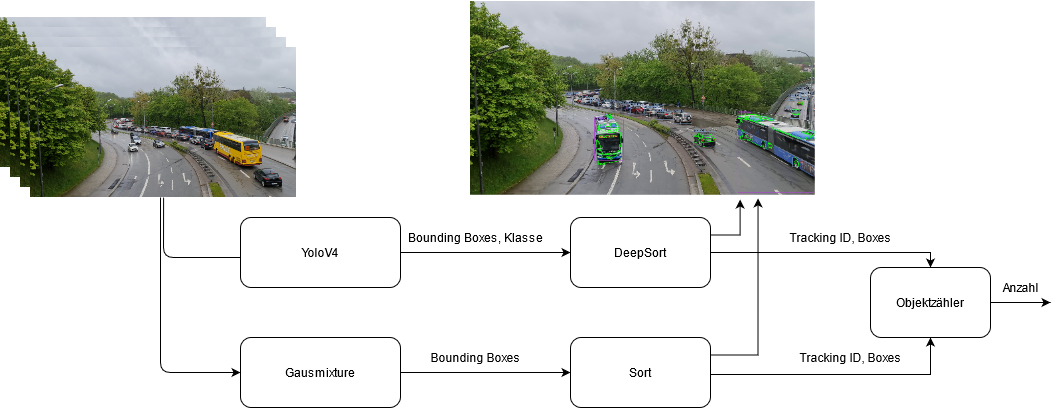
\includegraphics[width=14cm]{Media/KonzeptVAOT.png}
			\caption{Konzept für das Projekt}
			\label{Konzept}
		\end{center}
	\end{figure*}
	Ziel des Projektes ist es klassische Verfahren mit neueren DeepLearning Methoden zu vergleichen.
	Dafür ist für beide Arten eine Pipeline geschaffen worden.\\
	Für die Klassische Verfahren wurde für die Objekterkennung Gausmixture verwendet und für das Tracking Sort. Für die DeepLearning Verfahren wurde für die Objekterkennung ein Neuronales Netz  und für das Tracking wurde Deepsort verwendet. Mit einem Objektzähler können am Ende der Pipelines die Objekte gezählt oder mit einer Zustandserkennung die Bewegungen und Stillstand erfasst werden. Die Abbildung \ref{Konzept} visualisiert das Konzept.\\
	\\
	Bilder werden mittels OpenCV Bibliotheken Frame für Frame aus einem Video ausgelesen.
	Es ist möglich Bilder vor der weiteren Verarbeitung noch beliebig zuzuschneiden um nur relevant Bereiche zu betrachten. Dies hat den Vorteil das die Performance steigt und auch die Genauigkeit mancher Algorithmen zunimmt. Diese Bilder werden dann in die Pipeline gelegt.
	
	\section{Objekterkennung: Gauß Mixture}
	
	\subsection{Rauschminderung}
	
	\section{Objekterkennung: YoloV4}
	YOLO ist ein Neuronal Netz für die Echtzeit-Objekterkennung. YOLO ist die Abkürzung für 'You Only Look Once' was übersetzt 'Man sieht nur einmal hin' heißt. Die Aufgabe der Objekterkennung besteht darin, den Ort und die Bounding Box im Bild zu bestimmen, sowie die Objekte zu klassifizieren. Frühere Methoden, wie R-CNN und seine Variationen, verwendeten eine Pipeline, um diese Aufgabe in mehreren Schritten durchzuführen. Dies ist in der Ausführung langsam und aufwendiger zu trainieren, da jede einzelne Komponente separat trainiert werden muss. YOLO, erledigt beide Aufgaben mit einem einzigen Convolutional Neural Network. Es betrachtet dabei die Objekterkennung als ein Regressionsproblem auf räumlich getrennte Bounding Boxes und zugehörige Klassenwahrscheinlichkeiten.\cite{b1}\\
	Das Bild in ein S × S-Gitter mit den Residualblöcken aufgeteilt. Wenn der Mittelpunkt eines Objekts in eine Gitterzelle fällt, ist diese Gitterzelle für die Erkennung dieses Objekts zuständig. Jede Gitterzelle sagt B Bounding Boxes und C Klassen Konfidenzwerte für diese Boxen voraus \cite{b1}\\
	Diese Klassen Konfidenzwerte zeigen, wie sicher das Modell ist, dass die Boundingbox ein Objekt enthält und auch wie genau die Box das Objekt beschreibt. Die Konfidenz wird wie folgt definiert:
	\[ c = Pr(Objekt) * IoU_{pred}^{truth} \]
	Die IoU ist zwischen zwei Boxen A und B ist wie folgt definiert:
	\[ IoU = \frac{A \cap B}{A \cup B} \]
	Jede Boundingbox enthält die 5 Vorhersagen: x,y,w,h,c.
	Jede Gitterzelle sagt auch bedingte Klassenwahrscheinlichkeiten $Pr(Class_{i}|Object)$, voraus.  Diese Wahrscheinlichkeiten beziehen sich auf die Gitterzelle, die ein Objekt enthält.
	Zum Testzeitpunkt wird die bedingten Klassenwahrscheinlichkeiten und die individuellen Box-Vertrauensvorhersagen multipliziert, wodurch wir klassenspezifische Vertrauenswerte für jede Box erhalten.  Diese Werte kodieren sowohl die Wahrscheinlichkeit, dass diese Klasse in der Box vorkommt, als auch, wie gut die vorhergesagte Box zum Objekt passt.
	\[ Pr(Class_{i}|Object)*Pr(Object)*IoU_{truth}^{pred}= Pr(Class_{i})*IoU_{truth}^{pred} \]
	........Netzwerk???...........
	........LossFunction???...........
	
	In YoloV2 wurden Ankerboxen eingeführt. Da Objekte meist immer ähnliche Formen haben kann man eine gewisse Menge an sogenannten Ankerboxen definieren welche als Basis Boundingboxen fingieren. So wird anstatt die absolute Größen von Boxen in Bezug auf das gesamte Bild vorherzusagen, eine Ankerbox ausgewählt die am besten zu dem gewünschten Objekten passende verwendet. Die Abbildunf \ref{Anker} zeigt dieses Konzept.
	\begin{figure}[!h]
		\begin{center}
			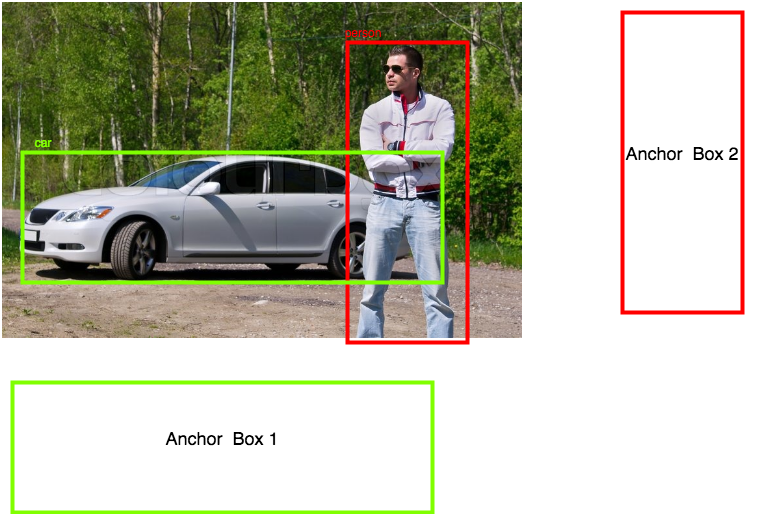
\includegraphics[width=6cm]{Media/Ankerboxen.png}
			\caption{Passende Ankerboxen werden ausgewählt\cite{b0}}
			\label{Anker}
		\end{center}
	\end{figure}
	Diese Ankerboxen kann man mittels Clusteralgorithmen wie K-Means und den Boundingboxen aus dem Datensatz berechnen werden. Dies hat vor allem den Vorteil das die Boundingboxenbesser zu den Objekten des jeweiligen Datensatzes besser passen. \cite{b3}\\ ++++++++BILD KMEANS ANKER+++++++
	.....
	YoloV3??
	YoloV4??
	....
	In diesem Projekt verwendeten wir die 4te und damit aktuell neueste Version von Yolo\cite{b2}. So bietet jede Version inkrementelle Verbesserung zum jeweiligen Vorgänger.\\
	Wir mussten unser Modell nicht mehr trainieren da es bereits mit dem Microsoft COCO Datensatz trainiert wurde. Es sind 80 verschiedene Klassen erkennbar. Wir interessieren uns aber nur für einen kleineren Teil wie:
	\begin{enumerate}
		\item Personen
		\item Pkw
		\item Lkw
		\item Busse
		\item Fahrräder
		\item Züge
	\end{enumerate}
	Das Modell könnte noch besser arbeiten wenn es nur auf die Klassen trainiert würde die für unser Projekt relevant sind. Dies hätte aber den Rahmen des Projektes gesprengt.\\
	Deshalb lassen sich je nach Szenario per Parameter die relevanten Klassen auswählen. Das Modell prädiktiert trotzdem noch alle Klassen. Die nicht relevanten werden einfach nur Postprocessing herausgefiltert.\\
	Ein weitere Postprocesingschritt ist es die Detektion die eine zu geringe Sicherheit besitzen zu entfernen.\\
	Die übrigen Boxen durchlaufen eine Non-Maxima-Suppression.
	Der Output kann überschneidende Boundingboxen besitzen die eigentlich zur selben Klasse gehören. Diese Duplikate können mittels der Non-Maxima-Suppression entfernt werden. Hierfür wird die IOU der Boxen berechnet. Sollte die IOU einen Threshold überschreiten dann wird das Duplikat entfernt. Die Grafik \ref{NMS} zeigt wie zu viele überlappende Boxen durch eine ersetzt werden.\\
	\begin{figure}[!h]
		\begin{center}
			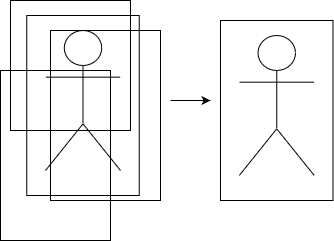
\includegraphics[width=6cm]{Media/NMS.png}
			\caption{Non-Maxima-Suppression}
			\label{NMS}
		\end{center}
	\end{figure}\\
	Das Ergebnis einer Prädiktion ist eine Liste von Objekten welches aus den x,y Koordinate des Mittelpunktes der Boundingbox, der Breite w, der Höhe h, der Klasse und des Konfidenzwerts besteht.
	
	\subsection{Fehler in der Erkennung}
	BRUDERMÜHL / ZUG FEHLT
	
	YoloV4 ist nicht perfekt. So gibt es gelegentlich Fehler:
	\textbf{Falschklassifizierung:}\\
	Selten Klassifiziert das Netz falsch. So wie in der Abbildung \ref{FaK} zu sehen ist wurde ein Bus als Pkw klassifiziert. Das Modell ist sich in diesem Beispiel auch nur unsicher mit $31\%$. Der Fehler lässt sich vermutlich erklären da die Frontpartie des Bus einem Pkw sehr ähnelt und der Rest des Fahrzeuges wegen einem Baum und einer Laterne verdeckt wird.
	\begin{figure}[!h]
		\begin{center}
			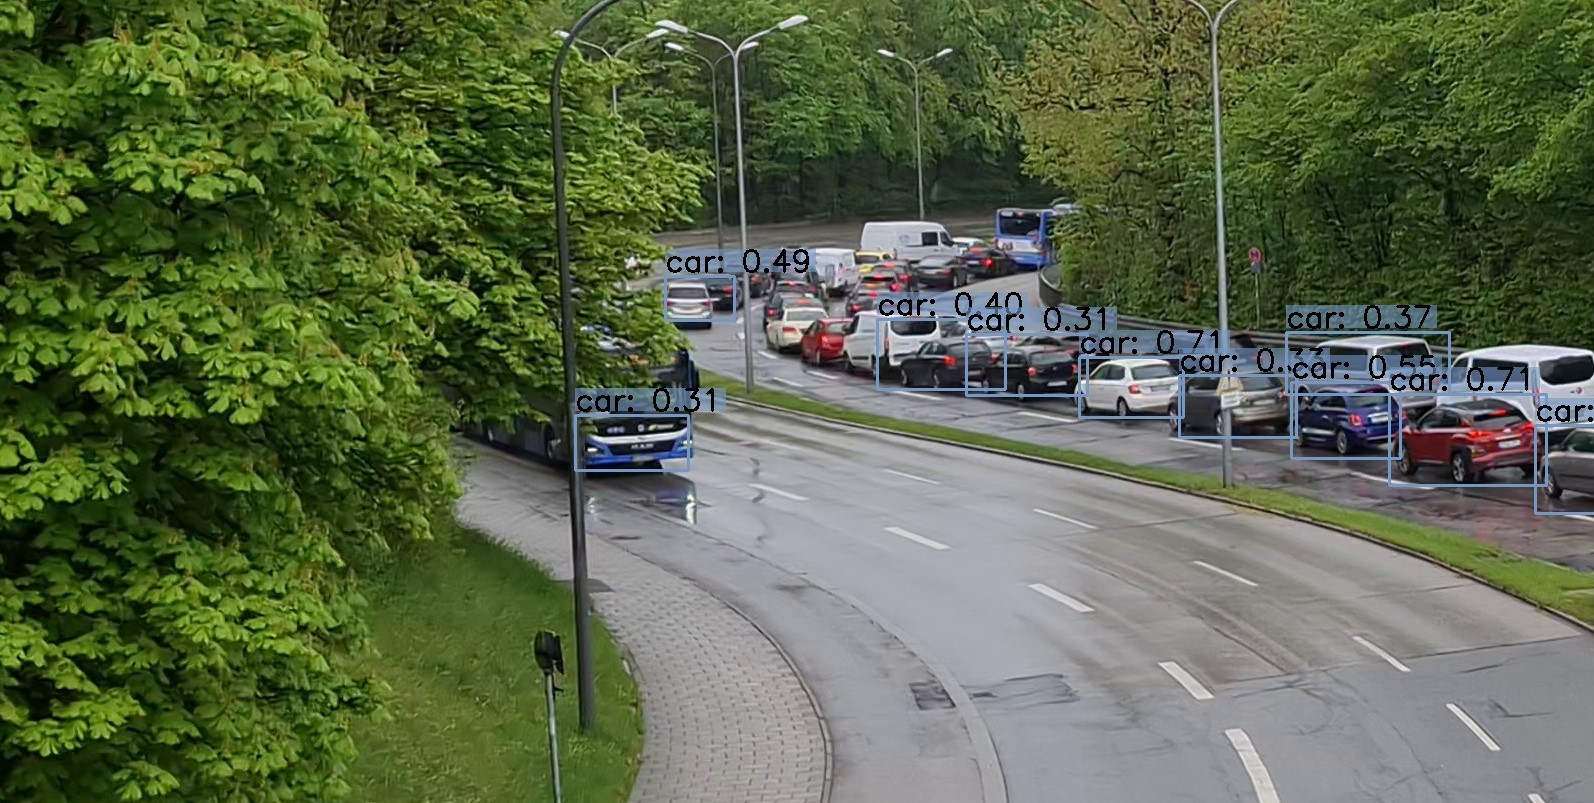
\includegraphics[width=7cm]{Media/Output_480 - Kopie.jpg}
			\caption{Falschklassifizierung}
			\label{FaK}
		\end{center}
	\end{figure}\\
	Außerdem DATENSATZ+++++++++++++++
	\begin{figure}[!h]
		\begin{center}
			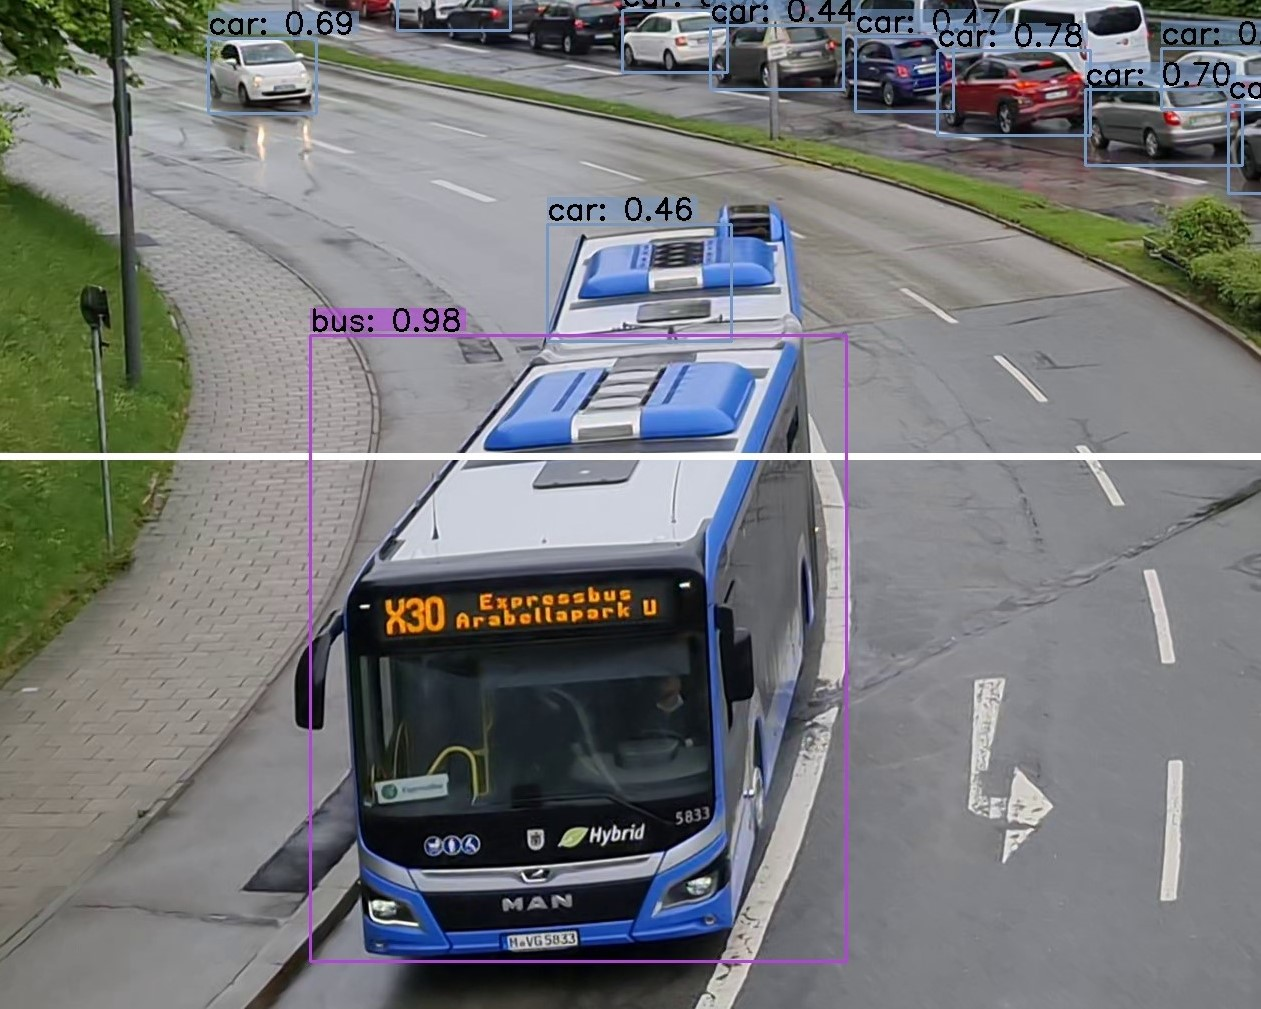
\includegraphics[width=7cm]{Media/Output_847 - Kopie.jpg}
			\caption{Falschklassifizierung}
			\label{FaK2}
		\end{center}
	\end{figure}\\
	\begin{figure}[!h]
		\begin{center}
			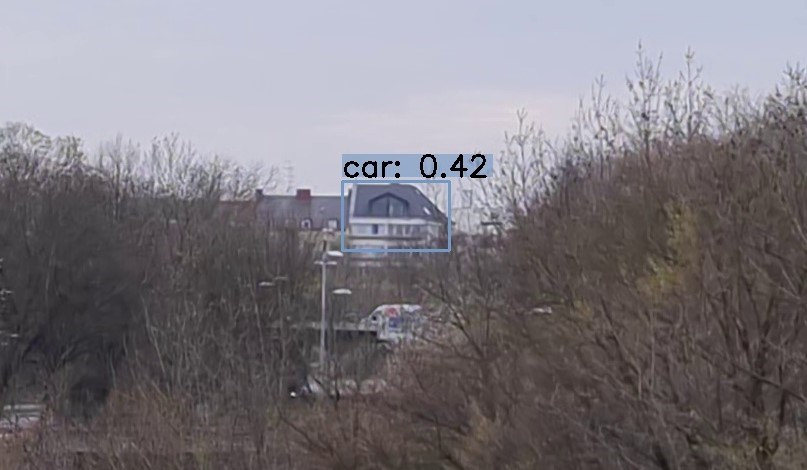
\includegraphics[width=7cm]{Media/Output_108 - Kopie (2).jpg}
			\caption{Falschklassifizierung}
			\label{FaK3}
		\end{center}
	\end{figure}\\
	\begin{figure}[!h]
		\begin{center}
			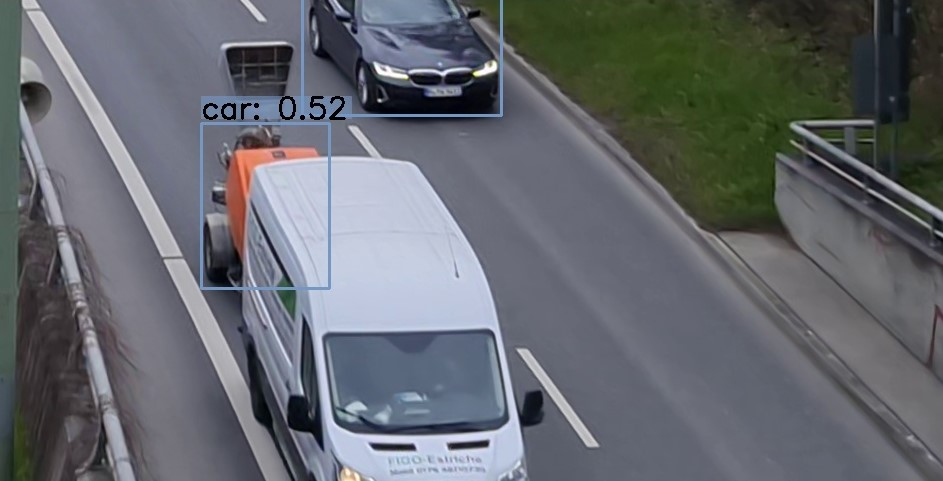
\includegraphics[width=7cm]{Media/Output_829 - Kopie.jpg}
			\caption{Falschklassifizierung}
			\label{FaK3}
		\end{center}
	\end{figure}\\

	\textbf{Fehlende Klassifikationen:}\\
	Ein etwas häufigerer Fehler ist das Klassifikationen Fehlen. Dies kann mehrere Gründe haben. So zeigt die Abbildung \ref{Fek} zwei Typische Gründe. Grund Nummer eins ist es das Objekte teilweise verdeckt sind. In Kombination wenn Objekte sehr klein sind ist es nahezu nicht mehr möglich zuverlässig Detektion zu bekommen. INPUT NETZ YOLO? Zu grobes GRID?? 
	\begin{figure}[!h]
		\begin{center}
			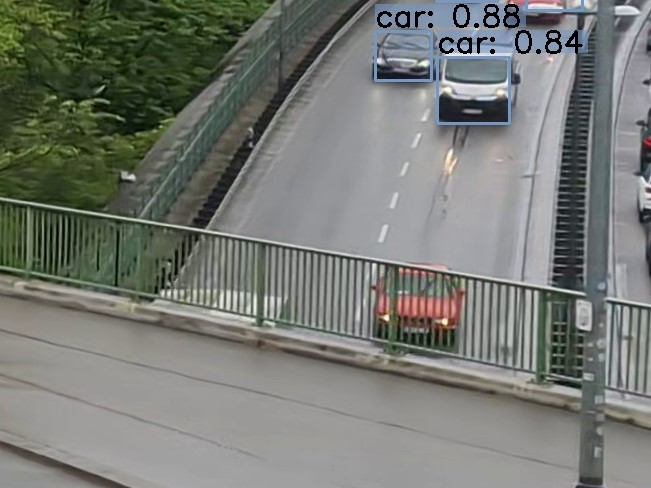
\includegraphics[width=7cm]{Media/Output_680 - Kopie.jpg}
			\caption{Fehlende Klassifikationen}
			\label{FeK}
		\end{center}
	\end{figure}\\
	\begin{figure}[!h]
		\begin{center}
			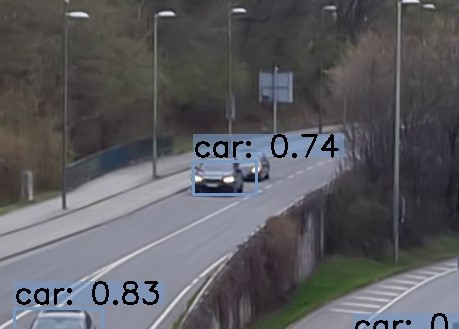
\includegraphics[width=7cm]{Media/Output_108 - Kopie.jpg}
			\caption{Fehlende Klassifikationen}
			\label{FeK2}
		\end{center}
	\end{figure}\\
	\textbf{Unpassende Boundingboxen:}\\
	Yolo hat eine große schwäche da es nur rechteckige Boundingboxen vorhersagen kann. Das resultiert in manchen Szenarien zu sehr unpassenden Boundingboxen. Beispielsweise kann man in der Abbildung \ref{UB} gut erkennen das wegen dem Bus welcher Diagonal steht die Boxen zu groß werden. Das selbe gilt für noch längere Objekte wie die Züge.++++++++ZUG BILD++. Auch kann die Box für das Objekt etwas falsch anliegen wenn Bäume oder Laternen ein Teil verdecken.
	\begin{figure}[!h]
		\begin{center}
			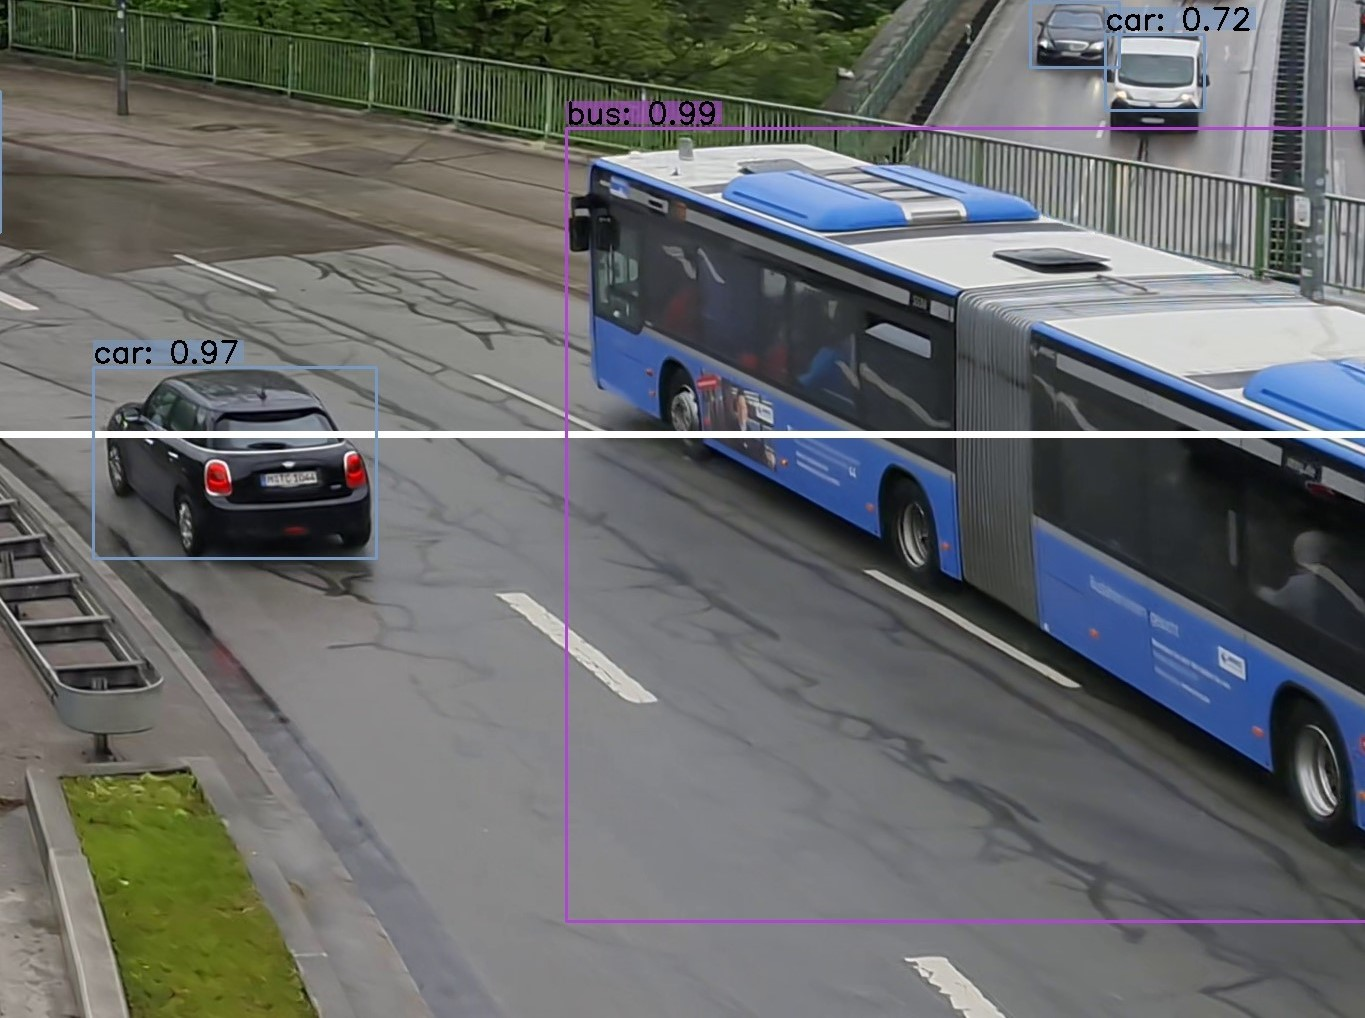
\includegraphics[width=7cm]{Media/Output_777 - Kopie.jpg}
			\caption{Unpassende Boundingboxen}
			\label{UB}
		\end{center}
	\end{figure}\\
	\begin{figure}[!h]
		\begin{center}
			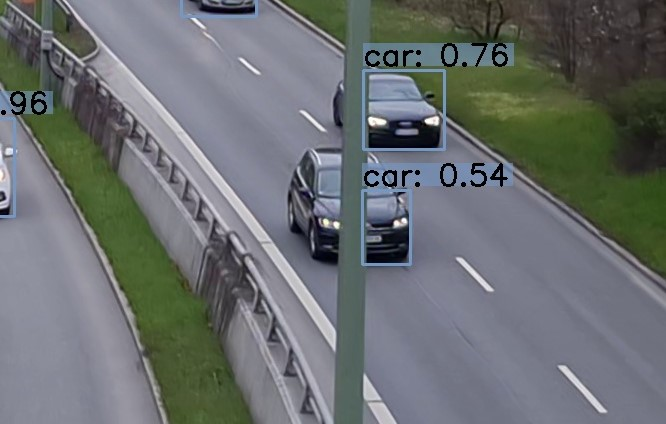
\includegraphics[width=7cm]{Media/Output_276 - Kopie.jpg}
			\caption{Unpassende Boundingboxen}
			\label{UB2}
		\end{center}
	\end{figure}\\

	...falsch Klassifizierung wegen schlechter Datensatz....
	Zu großer Datensatz...
	
	YOLO besitzt starke räumliche Beschränkungen für die Boundingbox-Vorhersagen, da es pro Gitterzelle nur eine begrenzte Anzahl an Vorhersagen treffen kann. Diese Anzahl ist direkt Abhängig von der Anzahl der Ankerboxen \cite{b3}. Diese räumliche Beschränkung begrenzt die Anzahl der Objekte in der Nähe, die das Modell vorhersagen kann. 
	-------------Problem zu viele Elemente nebeneinander..... wegen zu großen maschigen Grid zu wenig Ankerboxen????--------------

	\section{Tracking: Sort}
	SORT berechnet auf Basis des Kalman Filters und der Hungarian Methode die Bewegung des Objekts und weist je nach Status eine eindeutige Identifikationsnummer zu. Der Kalman-Filter funktioniert für die Problemstellung sehr gut, da dieser ein lineares System mit gaußisches Rauschen voraussetzt. Dies ist gegeben durch die gleichmäßige Bewegung der Züge/ Autos in eine Richtung.
	Der Kalmanfilter kann aus verrauschten, teils redundanten Messungen die Zustände und Parameter des aktuellen Systems schätzen. Die Zustände des aktuellen Systems sind die Positionen angegeben in Bounding Boxen der Objekte. Durch Berücksichtigung des letzten Zustand des Systems, (die letzte Position), der Schätzung der nächsten Position und Abgleich mit der aktuellen Messung (die aktuelle Detektion) und anschließender Aktualisierung des Systems, kann eine zuverlässige Verfolgung des Objekts berechnet werden. Probleme die den Kalmanfilter stören sind zum Beispiel ungleichmäßige Bewegungen von Fahrzeugen, dies wird „Process Noise“ genannt, sowie Ungenauigkeiten in Messungen, diese werden als „Measurement Noise“ bezeichnet.
	Kann für zu dem aktuell getrackten Objekt in dem Frame keine Bounding Box zugeordnet werden, wird der Zustand des Systems auch ohne die Korrektur durch die Messung berechnet und kann verwendet werden, sollte in einem späteren Frame wieder eine Bounding Box zugeordnet werden können. 
	Die Hungarian Methode wird verwendet um die Detektion einem existierenden Objekt zuzuorden. Hierfür wird die Intersection-over-Union Distance zwischen jeder Detektion und allen bereits erkannten Objekten verglichen. Die Assoziationsmatrix kann optimal durch die Hungarian Methode berechnet werden. Als Verbesserung wurde hier bei der Implementierung durch DeepSort noch eine Mindestüberschneidung $IoU_{min}$ eingeführt.
	
	
	\section{Tracking: DeepSort}
	
	SORT an sich ist bereits ein Tracker, das Problem ist jedoch, dass die ID-Änderungen zu oft auftreten. Das heißt die Objekt-ID wechselt während der Verfolgung. Ausgelöst wird dies zum Beispiel durch die teilweise Verdeckung des Objekts. Deshalb wurde SORT um ein CNN erweitert, welches sowohl einerseits die Mahalanobis-Distanzmetrik für die Assoziation nutzt, als auch die Form des Objekts in Form eines durch das hinzugefügte CNN berechneten Feature-Vektor verfolgt. Durch Verwendung einer geeigneteren Distanzmetrik und Beschreibung des Objekts kann dieses nun besser verfolgt werden.
	Das CNN erstellt einen Vektor, der enthält alle Features eines gegebenen Bilds. Ursprünglich wird das Neuronale Netz als Klassifikator trainiert. Indem die Klassifikations Layer weggelassen werden, können die resultierenden Feature-Vektoren als Wiedererkennungsform verwendet werden.
	
	Anstatt bei der Ungarischen Methode wie bei SORT die IoU-Distanz zu verwenden, wird nun die (quadrierte) Mahalanobis Distanz verwendet, welche die Distanz zwischen der detektierten Bounding Box und der gaußverteilten Vorsage des Zustands des Kalman-Filters berechnet:
	\begin{align}
	d^{(1)}(i,j)= (d_j - y_i)^TS^{-1}_i(d_j - y_i)
	\end{align}
	Hierbei wird die Verteilung, zuvor acht-dimensional des i-ten verfolgen Objekts in den vier-dimensionalen Raum der Messungen projiziert $(y_i, S_i)$. Diese Bounding Box der Detektion wird mit $d_j$ bezeichnet. \\
	
	
	\begin{tabular}{r l}
		Kalman-Filter Zustand: & $(u,v,\gamma,h,\dot{x},\dot{y},\dot{\gamma},\dot{h})$ \\
		Detektion: & $(u,v,\gamma,h)$ \\
		$u,v$ :& Mittelpunkt der Bounding Box \\
		$h$ :& Skalierungsfaktor \\
		$\dot{x},\dot{y},\dot{\gamma},\dot{h}$: & Geschwindigkeiten in Bild- \\	
		& koordinaten \\
	\end{tabular} \\

	Die Mahalanobis Distanz berechnet den Abstand von einem Punkt zu einer Verteilung. Der Abstand ist dabei wie viele Standardabweichungen der Verteilung dieser Punkt vom Mittelwert der Verteilung entfernt ist. Er wird somit durch die Standardabweichung der Verteilung normiert. Die Detektion stellt hierbei den Punkt da und die Unsicherheit der Zustandsvorhersage, beziehungsweise die Unsicherheit der Position des getrackten Objekts, die Verteilung. Dadurch wird bei der Berechnung der Distanz die Unsicherheit der Position miteinbezogen.
	
	Für die Distanzmetrik ergibt sich dann folgende Gleichung
	$D = \lambda * D_k + (1-\lambda) * D_a$. Hierbei ist $D_k$ die Mahalanobis Distanz und $D_a$ die kleinste Kosinus-Distanz zwischen den Feature-Vektoren. $\lambda$ dient als ein Gewichtungsfaktor.
	
	Kann DeepSORT erfolgreich ein bereits verfolgtes Objekt zu einer Detektion assoziieren, wird anschließend eine TrackingID erstellt. Hierbei muss beachtet werden, dass im Zuge der Verbesserung von SORT weitere Sicherheiten eingebaut wurden. Ein neu getracktes Objekt erhält nicht sofort eine endgültige Identifikationsnummer. Erst nachdem das Objekt in drei hintereinander liegenden Frames erfolgreich getrackt werden konnte erhält es eine Nummer. Das Objekt erhält des weiteren einen Zähler $a$, der die Anzahl an Frames zählt, seitdem das Objekt nicht mehr erfolgreich assoziiert werden konnte. Ist eine maximale Anzahl $Age_{max}$ erreicht gilt das Objekt als verloren oder außer Reichweite der Kamera und wird aus der Objektliste entfernt. Dieser Zähler wird jedoch zurückgesetzt, sollte zuvor das Objekt erneut erfolgreich assoziiert werden.
	
	\section{Zählen von Objekten}
	Wir testeten verschiedene Verfahren zu Zählen der gefundenen Objekte die das Video passieren.\\
	\textbf{Zählen der vergebenen TrackingID's.} Unser erster Plan war das Zählen aller vergebenen Tracking ID's. Dies hätte den Vorteil das sobald ein Objekt gefunden wird auch gezählt wird. Wir stellten aber schnell fest das Aufgrund von Fehlern in der Pipeline Objekten mehrfach neue IDs zugewiesen wurde. Diese Probleme entstehen in Kombination aus Fehlern in der Objekterkennung und dem Tracker. Je zuverlässiger das Tracking funktioniert desto geringer ist der Fehler im Zählen. Da aber ein perfekter Tracker nicht immer realistisch ist müssen bessere Lösungen gefunden werden.\\
	\textbf{Zähllinie.} Um Trackingfehler zu umgehen bauten wir eine Zähllinie ein die sobald der Mittelpunkt der Boundingbox diese schneidet einmal hochzählt. Dies hatte noch immer Probleme wie zum Beispiel das manche Boxen doppelt gezählt wurden ohne manche die Linie direkt übersprungen haben. WAS WAR DA NOCHMAL FALSCH Thomas?\\
	\textbf{Zählung der Tracking IDs in einer Zählbox.} Um die beiden Techniken zu vereinen wurde eine Zählbox entwickelt. So kann für jedes Szenario per Parameter die Position und Größe der Zählbox definiert werden. Sobald der Mittelpunkt einer Boundingbox in den die Zählbereich eindringt wird überprüft ob diese Tracking ID schon in einem Set enthalten ist. Ist sie es noch nicht wird hochgezählt. Es ist sinnvoll die Zählbox in Bereiche zu setzten in denen das Tracking zuverlässig funktioniert. 
	\begin{figure}[!h]
		\begin{center}
			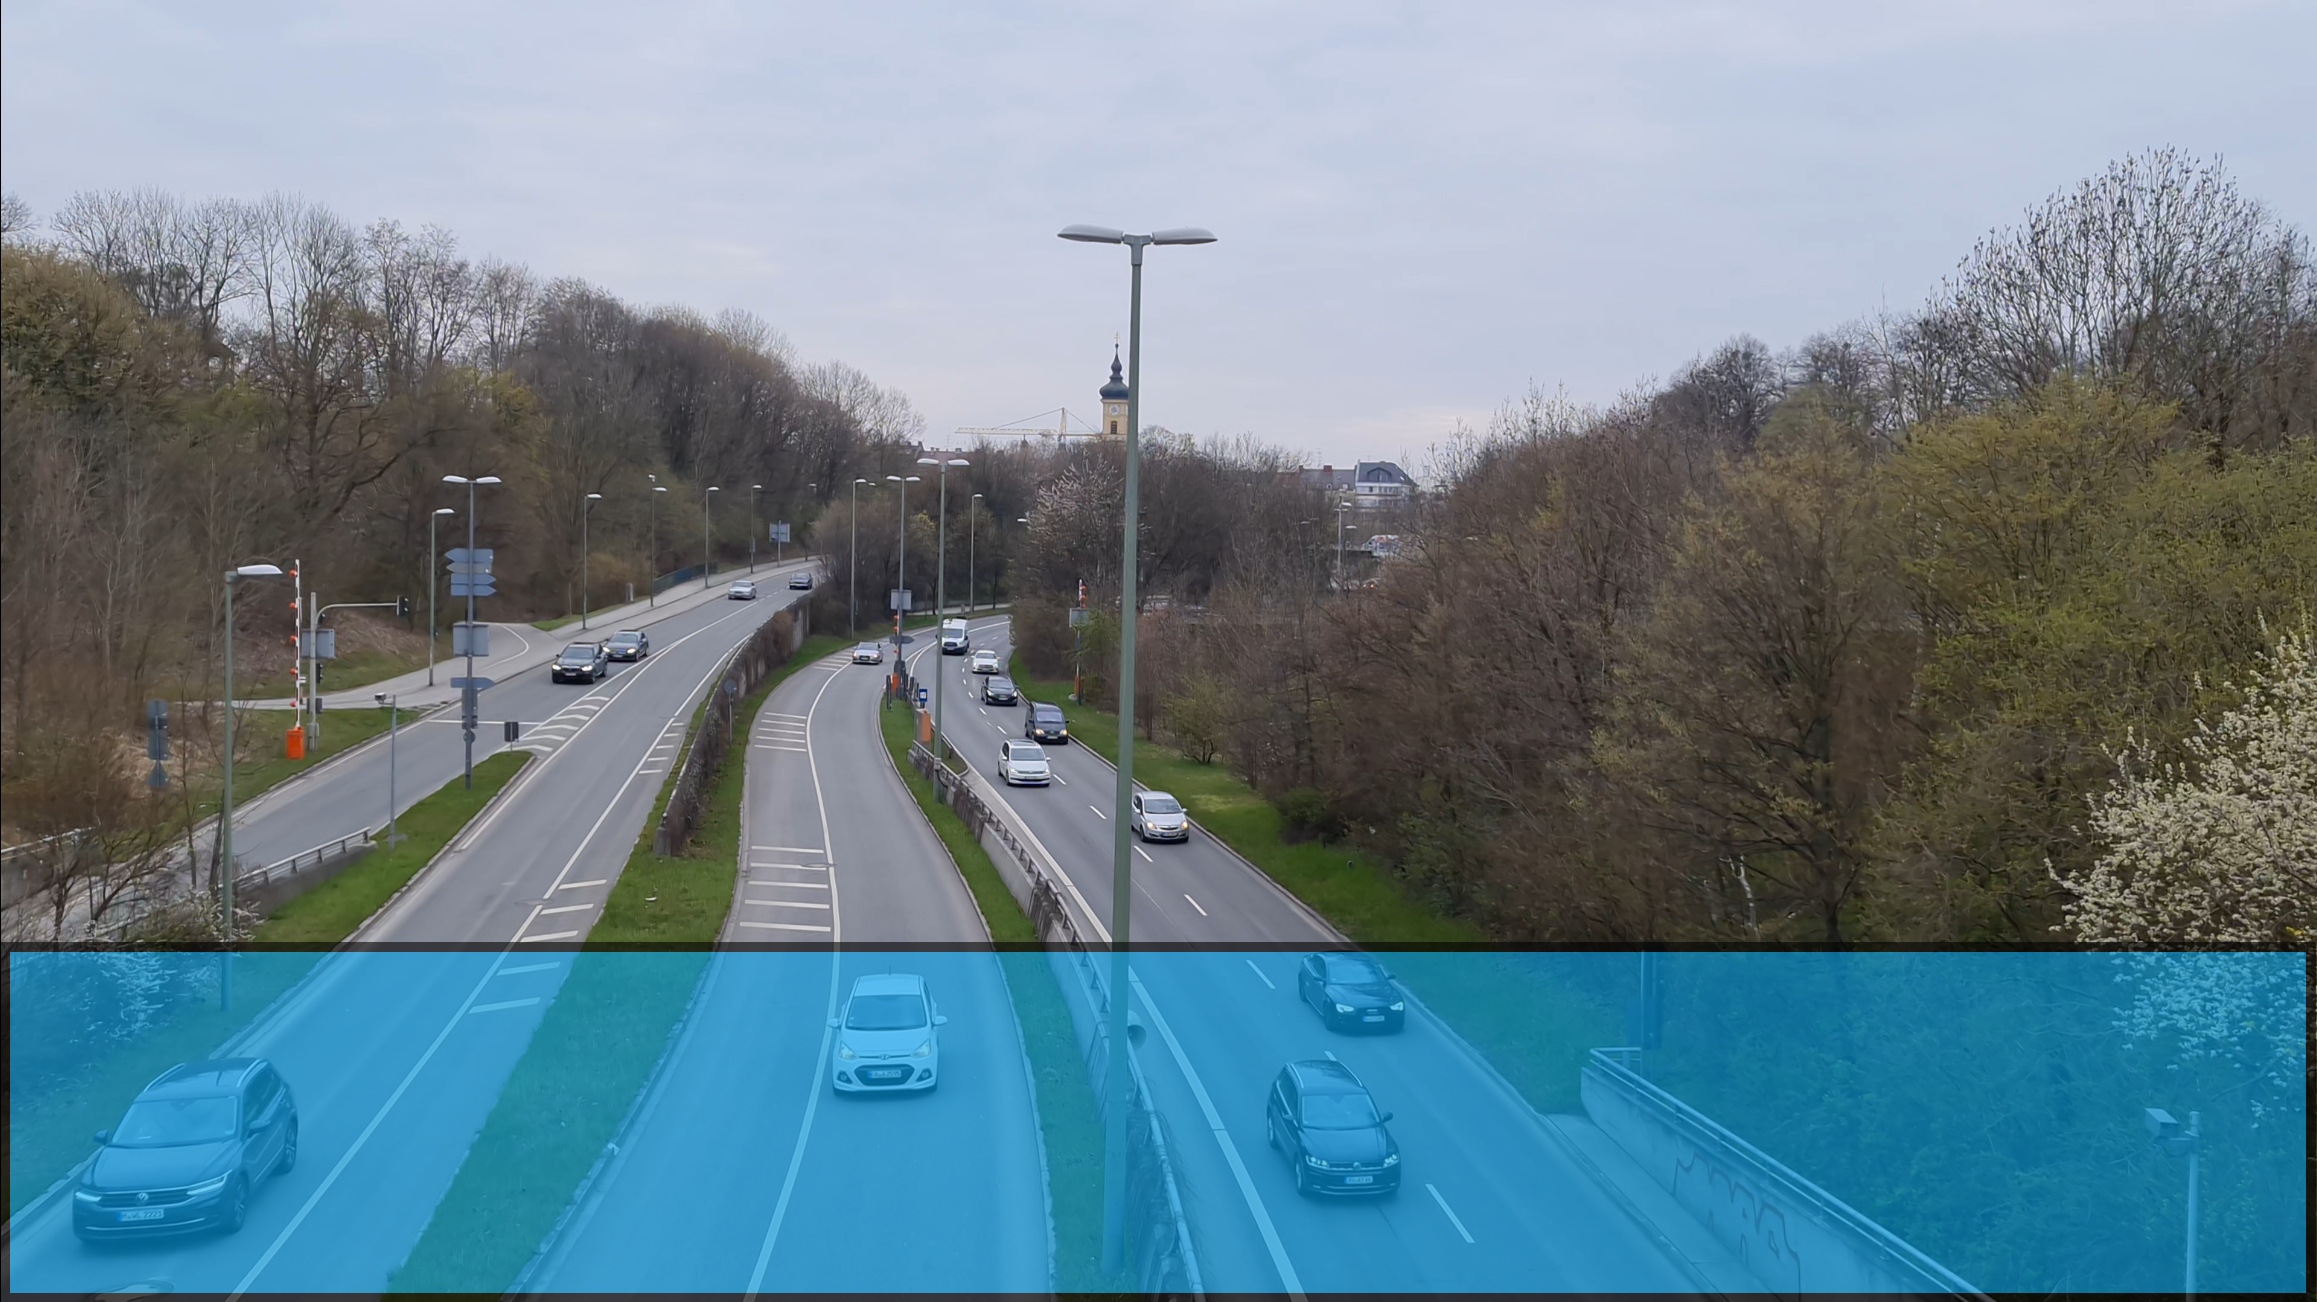
\includegraphics[width=7cm]{Media/BrudermuhlCounter.png}
			\caption{Darstellung einer Zählbox}
			\label{Counter}
		\end{center}
	\end{figure}
	
	\section{Zustandserkennung Züge}
	Da nun ein Objekt erfolgreich erkannt, verfolgt und seine Bewegungsrichtung erkannt werden kann, wird nun für Objekte die der Klasse Zug zugeordnet sind, die aktuelle Zugphase bestimmt.  
	Durch YOLO werden die Bounding Boxen pro Frame bestimmt. Durch Abgleich der TrackingID kann festgestellt werden, ob es sich immer um den selben Zug handelt. Für jede der Detektionen des ausgewählten Zugs wird durch Optical Flow die Magnitude und die Richtungswinkel bestimmt. Dabei wurde die durchschnittliche Richtung über die gesamten Richtungsvektoren der Bounding Box des Zuges bestimmt. Dies wurde im Verlauf des Projekt durch die Richtungsbestimmung des Kalmanfilters ersetzt. Dieser berechnet zusammen mit dem nächsten Zustand auch die den Richtungsvektor. Fährt der Zug ein, hat dieses Objekt durch die Bewegung eine Magnitude größer 1. Der Richtungsvektor wird zur Visualisierung in das Bild als Pfeil eingefügt. Sobald der Zug erkannt wird und eine Richtung bestimmt wird, wechselt dessen Zustand von „Kein Zug“ zu „Einfahrend“. Dabei wird immer für 5 Frames geprüft ob die Richtung gleichbleibend ist. Sollte für eine Länge von 10 Frames die Magnitude unter 0 fallen ändert sich der Zustand des Zuges zu „Haltend“. Beginnt der Zug sich wieder zu bewegen und die Bewegung ist gleichbleibend in eine Richtung wird der Zustand auf „Abfahrend“ gesetzt, bis der Zug außerhalb des Bildes ist und nicht mehr erkannt wird.
	
	\begin{thebibliography}{00}
		\bibitem{z1}https://www.zeit.de/news/2020-10/18/s-bahn-stammstrecke-in-muenchen-fuer-arbeiten-gesperrt
		\bibitem{b0}https://medium.com/@sarangzambare/object-detection-using-non-max-supression-over-yolov2-382a90212b51
		\bibitem{b1}https://arxiv.org/pdf/1506.02640v5.pdf
		\bibitem{b2}https://arxiv.org/pdf/2004.10934.pdf
		\bibitem{b3}https://arxiv.org/pdf/1612.08242.pdf
	\end{thebibliography}
	
	\section{Vergleich klassischen Methoden mit DeepLearning}
	
	\section{Anhang}
	

\end{document}
